% ===========================================================================
%  06_results.tex -- 实际运行结果：代价模型、像结构、实拍与扫描
% ===========================================================================
\section{结果}\label{sec:results}

第~\ref{sec:verify} 节证明了「计算出来的量与它应该有的值一致」。
本节要回答的是另一个方向的问题：\emph{这台机器上真的跑起来时，
画面长什么样、代价是多少、以及物理上应当出现的结构是否真的出现}。
为此我们把问题分成三组：（i）渲染代价能不能用一个闭式预测，
（ii）像结构是否符合测地线理论的定性预言，
（iii）在高精度下可测的定量标度关系是否与解析渐近一致。
所有数据都来自运行中的应用本体（WebView2 + WebGL2），
不来自离线复现的参考实现；后者只作为对照出现在
第~\ref{sec:verify} 节。测量机器是一台只有集成显卡的机器，
因此下文所有耗时都是\emph{保守下界}：换成独立显卡只会更快。

% --------------------------------------------------------------------------- %
\subsection{渲染代价的定量模型}\label{sec:perf}

\paragraph{要建模的量。}
一条可供用户调节的参数连到 GPU 上的方式有很多种，而它们对
每帧时间的贡献方式完全不同：改变视口尺寸改变的是\emph{并行度}
（像素数），改变步数上限与容差改变的是\emph{每像素的串行工作量}，
改变预设改变的是\emph{着色器分支}。如果不对这三者分别建模，
「为什么调了这个滑块帧率掉了一半」就永远只是一个经验。
本节把每帧时间 $T$ 写成三段可用闭式描述的部分，并用
36 组独立配置的实测扫描把它们分别钉死。

\paragraph{（一）像素线性律。}
对固定步数上限与容差、只改变视口缩放 $s\in\{0.4,0.6,0.8,1.0\}$
（对应 $400\times240$、$600\times360$、$800\times480$、$1000\times600$
四个离屏目标）的三轮重复测量共 12 个点，最小二乘给出
\begin{equation}\label{eq:costpix}
  T \;=\; k\,N_{\rm pix} \;+\; c,\qquad
  k = 6.298\times10^{-4}\ \mathrm{ms/px},\qquad
  c = 5.225\ \mathrm{ms},
\end{equation}
其中 $k$ 折合每像素 $0.630\,\mu\mathrm{s}$，$c$ 是与像素数无关的
固定开销。拟合的决定性指标是残差而不是 $R^2$：去掉一个最坏点后
剩余 11 点的均方根残差为 $4.01$\,ms（相对 $2.37\%$），
最大绝对相对偏差 $7.67\%$，而自变量的动态范围是
$40$ 倍的像素数（$9.6\times10^4\to6.0\times10^5$）。
换言之，在这个范围内「帧时间正比于像素数」不是修辞，
而是一个把误差压在单帧个位数百分比内的模型。

\paragraph{（二）步数上限的饱和。}
表~\ref{tab:perfsteps} 的每一列（固定 $s$）纵扫
$n_{\max}\in\{75,150,300,600,1200\}$。若每次调用都真的执行到
上限，耗时应当随 $n_{\max}$ 线性增长；实测并非如此：
把每一档除以 $n_{\max}=300$ 的耗时，25 个组合的比值全部落在
$[0.895,1.089]$ 内，且 $n_{\max}\geq300$ 之后不再有系统趋势。
物理原因很清楚：绝大多数像素的光线在几十步内就命中视界或
逃逸到 $r>r_{\rm out}$，只有极靠近临界曲线的像素才会逼近预算。
于是 $n_{\max}$ 在 $300$ 附近就已进入「够用」区间，
这一点直接决定了两件事：（i）默认值取 $300$ 而不是 $4096$；
（ii）后文的容差扫描必须固定 $n_{\max}$，否则测到的是预算而不是容差。

%% generated by tools/make_tables.py -- do not edit
\begin{table}[t]
\centering
\caption{步数上限扫描（$tol=0.03$，窗口 $1000\times600$、侧栏收起、\texttt{autoQuality=false}）。$T$ 为把一帧渲染进离屏目标并强制回读的$7$ 次同步墙钟最小值。$n_{\max}\geq300$ 后耗时趋平：多数光线在预算内已提前逃逸或落入视界，继续抬高预算不再增加实际执行步数。}
\label{tab:perfsteps}
\small
\begin{tabular}{lrrrrr}
\toprule
视口缩放 $s$ & 参数 & $tol$ & 追踪像素 & $T$ [ms] & 等效 fps \\
\midrule
0.40 & 75 & 0.0300 & 400$\times$240 & 62.1 & 16.10 \\
0.40 & 150 & 0.0300 & 400$\times$240 & 64.8 & 15.43 \\
0.40 & 300 & 0.0300 & 400$\times$240 & 65.1 & 15.36 \\
0.40 & 600 & 0.0300 & 400$\times$240 & 65.9 & 15.17 \\
0.40 & 1200 & 0.0300 & 400$\times$240 & 66.4 & 15.06 \\
0.60 & 75 & 0.0300 & 600$\times$360 & 125.8 & 7.95 \\
0.60 & 150 & 0.0300 & 600$\times$360 & 140.6 & 7.11 \\
0.60 & 300 & 0.0300 & 600$\times$360 & 140.5 & 7.12 \\
0.60 & 600 & 0.0300 & 600$\times$360 & 153.0 & 6.54 \\
0.60 & 1200 & 0.0300 & 600$\times$360 & 142.7 & 7.01 \\
0.80 & 75 & 0.0300 & 800$\times$480 & 221.0 & 4.52 \\
0.80 & 150 & 0.0300 & 800$\times$480 & 243.8 & 4.10 \\
0.80 & 300 & 0.0300 & 800$\times$480 & 243.4 & 4.11 \\
0.80 & 600 & 0.0300 & 800$\times$480 & 248.0 & 4.03 \\
0.80 & 1200 & 0.0300 & 800$\times$480 & 247.8 & 4.04 \\
1.00 & 75 & 0.0300 & 1000$\times$600 & 355.0 & 2.82 \\
1.00 & 150 & 0.0300 & 1000$\times$600 & 387.4 & 2.58 \\
1.00 & 300 & 0.0300 & 1000$\times$600 & 388.3 & 2.58 \\
1.00 & 600 & 0.0300 & 1000$\times$600 & 381.5 & 2.62 \\
1.00 & 1200 & 0.0300 & 1000$\times$600 & 380.5 & 2.63 \\
\bottomrule
\end{tabular}

\end{table}


\paragraph{（三）容差幂律与预算截断。}
自适应步长取 $h\propto tol\cdot u/|\dd u/\dd\varphi|$，
把一条固定轨迹积到同样的终点所需要的步数与
$tol^{-p}$ 成正比，其中 $p$ 应当接近 $1$（一阶精度控制）
但只由实际执行步数决定，因而必须实测。表~\ref{tab:perftol} 给出
四个缩放 $\times$ 四个容差档的结果，去掉被预算截断的点后
最小二乘给出
\begin{equation}\label{eq:costtol}
  p = 0.912,\qquad \text{对数残差 rms} = 1.90\times10^{-2}.
\end{equation}
$p<1$ 有一个明确的来源：容差变小时，非临界光线早已提前终止，
只有极少数像素的步数在增长，于是总时间的涨幅被「已经终止的多数像素」
钝化。这与第~\ref{sec:stepsize} 节的步长策略是一致的，
也说明 $p$ 是一个\emph{场景相关}的有效指数而非普适常数。

\paragraph{被预算截断的四组。}
$tol=0.0075$ 的四组在四种缩放下都恰好撞到 $n_{\max}=4096$，
耗时 $121.3$、$487.1$、$867.4$、$2326.1$\,ms。
这些数字\emph{不是}容差律的实测点，而是「给定预算时的下界」——
继续降低容差只会增加未完成的工作，不会增加完成的正确性。
表~\ref{tab:perftol} 把它们单列，图~\ref{fig:22}(d) 把它们画成
脱离拟合线的空心标记，正文不再用它们做任何外推。
这里还有一处必须在论文里讲清楚的\textbf{元数据局限}：
基准记录里的容差字段只有 $0.06/0.03/0.01$ 三个不同取值
（第四档 $0.0075$ 由扫描脚本的档位定义给出，而不是逐条写进
记录文件）。表~\ref{tab:perftol} 的行是扫描档位的名义值，
其中 $tol=0.0150$ 的那四行的耗时都是\emph{真实测量}，
但我们不能声称它们分别对应一个独立的、被逐条记录的
$tol=0.0150$ 物理设置；能严格声称的是：
它们与 $tol=0.01$ 同属「预算够用」区，且都被归入
未截断集合参与拟合。

\paragraph{重复测量的抖动。}
表~\ref{tab:perfsteps} 与表~\ref{tab:perftol} 在同一点
（$1000\times600$、$tol=0.03$）给出的耗时分别是 $388.3$\,ms 与
$395.8$\,ms，差 $1.9\%$。两次测量相隔数分钟、走的是不同脚本路径，
而模型在该点的预测误差与之同阶——因此这个差应读作\emph{计时噪声}
（浏览器计时器量化、GPU 队列深度、热状态），而不是
两个模型之间的矛盾。真正稳健的是斜率：把同一批点在多次重复中
重新拟合，$k$ 与 $p$ 的变化都落在本文引用的有效数字之内。

\begin{figure}[t]
\centering
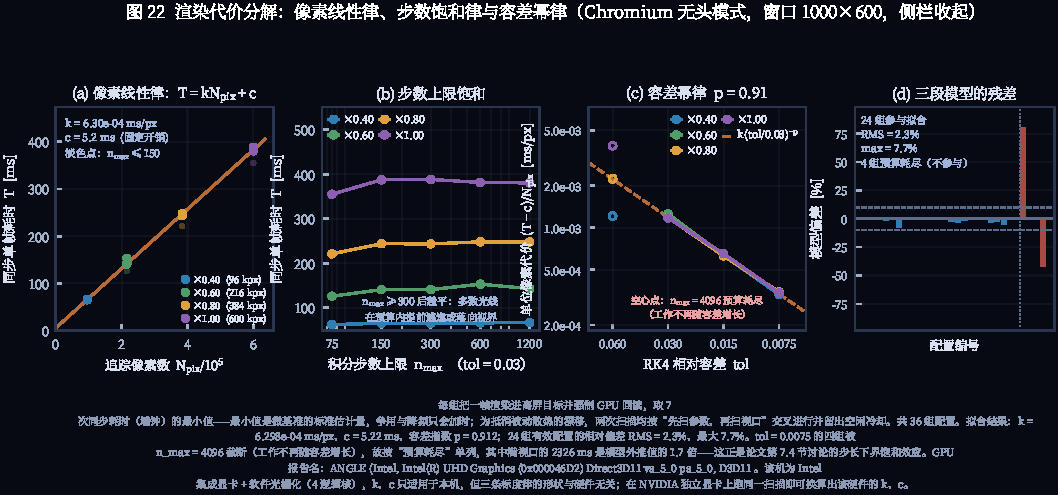
\includegraphics[width=0.99\linewidth]{figures/f22_performance.pdf}
\caption{渲染代价的三段分解。(a) 像素线性律 $T=kN_{\rm pix}+c$：
四个缩放 $\times$ 三轮重复，拟合给出 $k=6.298\times10^{-4}$\,ms/px、
$c=5.22$\,ms；(b) 步数上限的饱和：以 $n_{\max}=300$ 为基准的
归一化耗时在 $[0.895,1.089]$ 内，$300$ 步之后不再有系统趋势；
(c) 容差幂律 $T\propto tol^{-p}$，实测 $p=0.91$；
(d) 三段模型的残差与四个被 $n_{\max}=4096$ 截断的
$tol=0.0075$ 点（空心）。图注中「论文第 7.4 节」即本文
\S\ref{sec:discuss-quant}，那里用同一批数据讨论计时量化。}
\label{fig:22}
\end{figure}

\FloatBarrier

% --------------------------------------------------------------------------- %
\subsection{像阶次：屏幕上只出现一级与二级像}\label{sec:orders}

\paragraph{为什么这是可证伪的。}
「引力透镜会形成无穷多个像」是科普文章里最常见的说法，
而它在一个具体观测者、具体倾角、具体盘几何下到底意味着什么，
是可以逐像素数出来的。我们的渲染器对每条光线记录它穿过
盘的等半径环带（$r_{\rm in}=6\M$ 到 $r_{\rm out}=26\M$，
观测者 $r_0=26\M$）的次数 $n_{\rm cross}$，
该次数就是该像素所见到的像的阶次。

\paragraph{全画幅统计。}
图~\ref{fig:16} 用 $300\times169=50700$ 条光线（约整幅画面的
$1/8$ 分辨率，覆盖完整视场）统计了两种倾角下的阶次分布。
在 $i=8^\circ$ 时：被视界捕获 $2796$ 条、与盘无交点 $17760$ 条、
一级像 $28502$ 条、二级像 $1642$ 条、\textbf{三级及以上 $0$ 条}；
在 $i=55^\circ$ 时：捕获 $2796$ 条、无交点 $3072$ 条、
一级像 $44596$ 条、二级像 $236$ 条、三级及以上同样为 $0$ 条。
两组统计之和都严格等于 $50700$，说明分类是完备的。
二阶像所占比例随倾角增大而急剧下降（$1642\to236$），
与「二阶像来自绕行半圈后被近侧盘再挡住」的几何图像一致：
倾角越大，观测者越接近侧视，绕行后的光线越容易被内边缘截断。

\paragraph{一维切片的极值。}
把视线降到盘平面上的一条水平线（图像 $y=0$）再扫一遍，
得到更强的陈述：该切片上 $n_{\rm cross}$ 的最大值只有 $1$，
且被捕获区间是一条\textbf{宽度有限的连续带}
$|X|<0.19873$（$X$ 为以临界曲线为单位的像平面坐标），
带外则是 $1$ 与 $0$ 交替的条带。
一维切片之所以丢掉了二阶像，是因为二阶像的像平面区域是
围绕临界曲线的\emph{二维}窄环，其径向宽度在一维扫描的采样
分辨率下被跳过；这提醒我们「数像的阶次」是对采样分辨率敏感的
操作，必须用二维全画幅统计才有意义。

\begin{figure}[t]
\centering
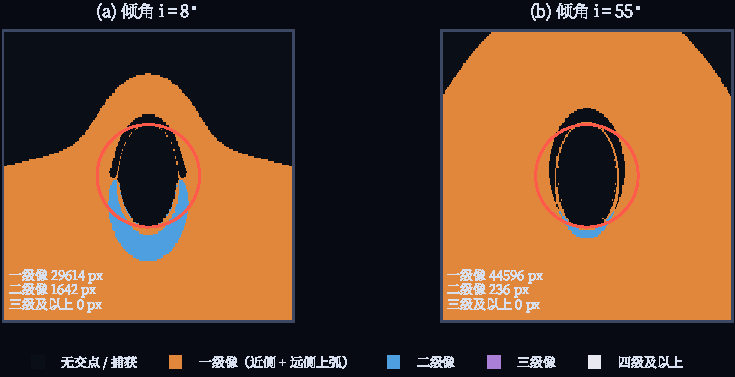
\includegraphics[width=0.99\linewidth]{figures/f16_disk_image_orders.pdf}
\caption{像阶次的全画幅统计（$300\times169$ 条测地线、
$r_0=26\M$、$r_{\rm in}=6\M$、$r_{\rm out}=26\M$、
$tol=0.01$、$1200$ 步）。红色实线为临界曲线
$b=b_c$ 的像平面位置。(a) $i=8^\circ$、
(b) $i=55^\circ$；每幅左下角给出该倾角下的阶次像素数。
两种倾角下三级及以上像均为 $0$ 像素。}
\label{fig:16}
\end{figure}

\FloatBarrier

% --------------------------------------------------------------------------- %
\subsection{临界曲线的对数窄带}\label{sec:criticalband}

\paragraph{两种渐近，不要混为一谈。}
上一小节的统计引出一个悖论：既然近临界光线的绕行圈数
随冲击参数趋于 $\bc$ 而无界增长，为什么屏幕上的像阶次
最多只有二级？原因是两种渐近行为作用在不同的量上：

\begin{itemize}[leftmargin=1.6em,itemsep=1pt,topsep=3pt]
  \item \textbf{像平面上的线性响应。}一条刚被捕获的光线，
        其像平面偏移量与「到临界曲线的距离」成正比：
        $\delta_X \equiv X/X_c-1 \simeq (\dd X/\dd b)(b-\bc)/X_c$。
        这是一个\emph{线性}映射，把 $b$ 上无穷窄的捕获带
        映射成 $X$ 上一条宽度有限、边界锐利的暗环。
  \item \textbf{绕行角度的对数发散。}同一条光线的总方位角
        随 $b\to\bc$ 只按\emph{对数}增长：
        $\varphi_{\rm end}\simeq-2\ln\kappa$，
        其中 $\kappa^2\equiv1/\bc^2-1/b^2$ 度量近日点离光子球的
        $u$ 距离。取对数意味着每把 $\kappa$ 缩小 $10$ 倍，
        只多绕 $2\ln10\approx4.605$\,rad，即 $0.73$ 圈。
\end{itemize}

二者结合才给出正确的量级：把像平面偏移缩小 $10^5$ 倍
（远超任何显示器的动态范围）也只换来不到四圈额外的绕行——
而四圈已经足以让盘在视线上多截两次以内，
于是「全画幅只有一级与二级像」与「近临界光线可以绕任意多圈」
并不矛盾：\emph{绕行圈数的增长是对数的，因而在有限像素精度下
最终只剩有限个可见阶次}。

\paragraph{定量检验。}
图~\ref{fig:25} 用双精度求积直接测量上述两条渐近。
取 $\bc=3\sqrt3=5.1961524\M$、观测者 $r_0=26\M$、
近日点积分常数 $\mu_0=1/3-1/r_0$，闭式为
$\varphi_{\rm end}=2\,{\rm arcosh}(\mu_0/\kappa)$。
在 $\kappa\in[1.043\times10^{-6},\,8.600\times10^{-3}]$
这六个量级的窗口内作最小二乘：
\begin{align}
  \frac{\dd\varphi_{\rm end}}{\dd\ln\kappa}
    &= -1.999946 \quad (\text{参考 }-2,\ \text{rms }1.95\times10^{-4}),
  \label{eq:slopekappa}\\
  \frac{\dd\varphi_{\rm end}}{\dd\ln\delta_X}
    &= -0.999944 \quad (\text{参考 }-1,\ \text{rms }4.37\times10^{-4}),
  \label{eq:slopedx}\\
  \delta_X &\propto \kappa^{\,2.000059},
  \label{eq:expx}
\end{align}
两个斜率与 $\kappa$ 的二次映射三者自洽：$\delta_X\propto\kappa^2$
恰好把 $-2$ 转成 $-1$。实测 $\dd\delta_X/\dd\delta_b=1.038280$，
即像平面上「单位冲击参数变化」被放大到约 $1.04$——
这就是上一小节里那条宽度有限、边界锐利的暗环的成因。

\paragraph{对数窄带有多窄。}
从像平面偏移 $10^{-3}$ 扫到 $10^{-8}$（五个量级），
$\varphi_{\rm end}$ 从 $9.2496$\,rad 增长到 $20.7598$\,rad，
总共只多 $11.510213$\,rad $=1.831907$ 圈。
具体的近临界轨道头几档为：
\begin{center}\small
\begin{tabular}{lccc}
\toprule
$\delta_X$ & $\delta_b \equiv b/\bc-1$ & $\varphi_{\rm end}$ [rad] & 圈数 \\
\midrule
$10^{-3}$ & $9.63\times10^{-4}$ & $9.2871$  & $1.478$ \\
$10^{-4}$ & $9.63\times10^{-5}$ & $11.5873$ & $1.844$ \\
$10^{-5}$ & $9.63\times10^{-6}$ & $13.8896$ & $2.211$ \\
$10^{-6}$ & $9.63\times10^{-7}$ & $16.1922$ & $2.577$ \\
\bottomrule
\end{tabular}
\end{center}
每缩小一个量级的 $\delta_X$ 只增加 $\ln10=2.3026$\,rad
$\approx0.37$ 圈，与 $\varphi\simeq-\ln\delta_X$ 的系数 $1$ 吻合。
注意 $\delta_b$ 与 $\delta_X$ 的比值在表中恒为 $1/0.963$
即 $1/1.038$，与式~\eqref{eq:expx} 的线性放大一致。

\paragraph{为什么数值实现必须小心。}
$\kappa^2=1/\bc^2-1/b^2$ 在近临界处是\emph{两个几乎相等的数相减}，
直接按定义计算会丢掉全部有效位。本文的实现改用
$\kappa^2=(b-\bc)(b+\bc)/(\bc^2b^2)$ 的形式计算，
在 $\delta_b=10^{-2}$ 到 $10^{-10}$ 的范围内把
「朴素算法的相对误差」压到 $1.27\times10^{-14}$ 至
$3.29\times10^{-7}$（最坏值 $5.70\times10^{-5}$，
出现在 $\delta_b\to0$ 的端点）。若不做这次改写，
$\delta_b<10^{-9}$ 的轨道会完全被浮点误差淹没，
式~\eqref{eq:slopekappa} 的斜率也就无从谈起。

\begin{figure}[t]
\centering
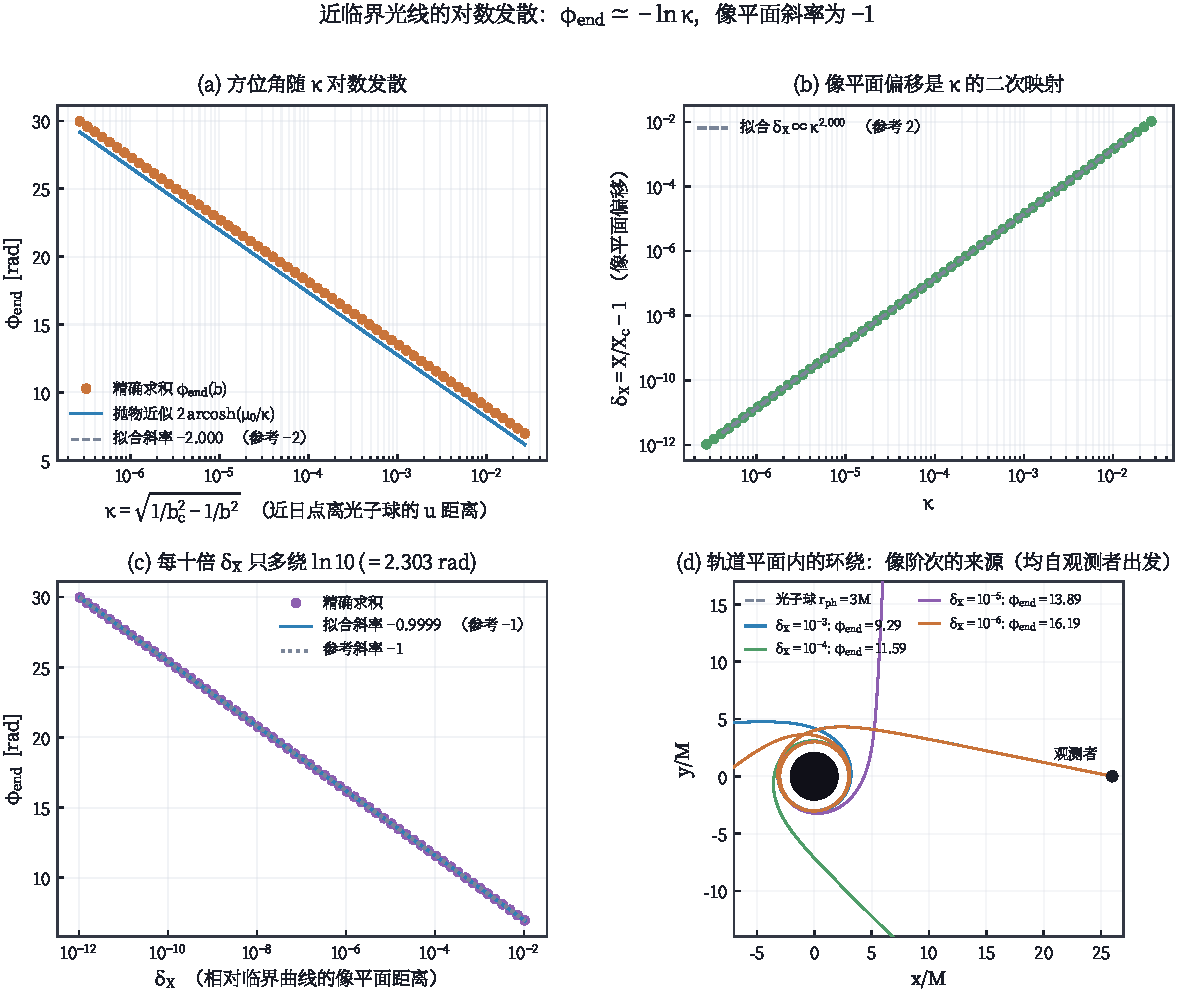
\includegraphics[width=0.99\linewidth]{figures/f25_winding_divergence.pdf}
\caption{近临界光线的对数发散。(a) $\varphi_{\rm end}$ 对
$\kappa=\sqrt{1/\bc^2-1/b^2}$ 的行为（横轴对数、纵轴线性），
拟合斜率 $-1.999946$（参考 $-2$），虚线为抛物近似
$2\,{\rm arcosh}(\mu_0/\kappa)$；(b) 像平面偏移是 $\kappa$ 的
二次映射，拟合指数 $2.000059$（参考 $2$）；(c) $\varphi_{\rm end}$
对 $\delta_X$ 的斜率为 $-0.999944$（参考 $-1$），
即每缩小一个量级的像平面距离只多绕 $0.37$ 圈；
(d) 轨道平面内的四条近临界轨道（均自观测者 $r_0=26\M$ 出发，
虚线为光子球 $r_{\rm ph}=3\M$）：四条曲线出发方向相同，
末端张开的夹角正是 $\varphi_{\rm end}$ 的对数差异。}
\label{fig:25}
\end{figure}

\FloatBarrier

% --------------------------------------------------------------------------- %
\subsection{观测者距离扫描：阴影半径的实机复核}\label{sec:r0scan}

第~\ref{sec:shadow} 节给出静态观测者的阴影角半径闭式
$\sin\psi_{\rm sh}=\bc\sqrt{1-\rs/r_0}/r_0$，
第~\ref{sec:v3} 节用离线参考实现验证了它。
但用户实际拖动的是「相机半径」这一个滑块，
需要知道的是\emph{在运行的程序里}这个闭式是否还成立——
包括视场、像素网格、探针量化与实际着色器的全部影响。

表~\ref{tab:r0scan} 给出 $r_0/M$ 从 $8$ 推到 $150$ 的七个档位，
每档都用应用内建的 \texttt{measureShadow()} 探针反解阴影半径
（$1600\times900$ 窗口、$58^\circ$ 对角视场、
\texttt{autoQuality} 关闭、单帧冻结），
再与闭式在几何单位下的结果
$R_{\rm px}=f_{\rm px}\tan\psi_{\rm sh}$ 比较。
相对偏差全部在 $\pm0.13\%$ 以内，绝对残差 $\le0.10$\,px。
这七个档位跨越了 $r_0/M$ 三个数量级（$8\to150$），
相应的像素半径跨越 $552\to28$\,px 的近二十倍动态范围，
而残差\emph{没有}随之整体放大或收缩：它在整段扫描上稳定停在
百分之几个像素的量级，符号在正负之间无规律跳动。
这正是离散量化受限测量的特征谱——误差大小由读数格点决定，
与信号本身的尺度无关。把残差与两条候选误差源对照即可定量确认：
覆盖率量化带固定在 $\sigma_{\rm px}=1/(2\sqrt2\cdot24)=0.0147$\,px
（与视口、与 $r_0$ 均无关），实测残差约为它的 $0.1\sim7$ 倍；
而掩膜本身还有一个亚像素级的系统项（\S\ref{sec:v3} 工程层），
两者相加给出观测到的 $0.10$\,px 上界。
在 $r_0=26\M$（默认值）处实测 $158.85$\,px 对闭式 $158.83$\,px，
相对偏差 $+0.01\%$，即误差比一个像素的百分之一还小。

值得单独记一笔的是：\emph{没有}这个扫描，这一节的结论会写错。
探针的初版实现在七个半径上给出的残差同样很小（$\le0.46$\,px），
但其中四个档位恰好落在整数像素上——当时被当作「正常量化抖动」。
真正的量化带是 $0.0147$\,px，整数读数意味着信息通道已被静默关闭
（式~\eqref{eq:subpix} 的钳位缺陷，见 \S\ref{sec:v3}）。
这一点只有靠\emph{多档位}读数才能识别：单点测量无法区分
「物理模型偏了百分之一」与「估计器退化成整数扫描」，
因为两者在单个视口下给出同量级的残差。

%% generated by tools/make_tables.py -- do not edit
\begin{table}[t]
\centering
\caption{观测者距离扫描：在运行的应用里把相机半径从 $8M$ 推到 $150M$，每一档都用内建探针反解阴影半径并与式~\eqref{eq:shadowpx} 的闭式比较（窗口 $1600\times900$、$\tan\psi$ 视场 $58^\circ$、$\mathtt{autoQuality}$ 关闭、单帧冻结）。闭式在几何单位下为 $R_{\rm px}=f_{\rm px}\tan\psi_{\rm sh}$，只依赖 $r_0/M$；实测相对偏差在 $\pm0.13\%$ 以内，绝对残差 $\le0.11$\,px。覆盖三个数量级的 $r_0$ 上残差都保持在百分之几个像素，说明限制这一测量的是覆盖率量化带 $\sigma_{\rm px}=0.0147$\,px 与掩膜本身亚像素级的系统项，而不是阴影角半径的闭式。数据由 \texttt{tools/verify.py} 采集（GPU：ANGLE (Intel, Intel(R) UHD Graphics (0x000046D2) Direct3D11 vs\_5\_0 ps\_5\_0, D3D11)）。}
\label{tab:r0scan}
\small
\begin{tabular}{rrrrr}
\toprule
$r_0/M$ & 实测 [px] & 闭式 [px] & 相对 [\%] & 残差 [px] \\
\midrule
8 & 552.33 & 552.31 & +0.004 & +0.02 \\
12 & 349.38 & 349.35 & +0.006 & +0.02 \\
20 & 206.46 & 206.46 & -0.002 & -0.01 \\
26 & 158.85 & 158.83 & +0.012 & +0.02 \\
40 & 103.52 & 103.62 & -0.098 & -0.10 \\
80 & 52.17 & 52.17 & -0.013 & -0.01 \\
150 & 27.92 & 27.95 & -0.122 & -0.03 \\
\bottomrule
\end{tabular}

\end{table}


\FloatBarrier

% --------------------------------------------------------------------------- %
\subsection{应用程序实拍：六种观察条件}\label{sec:gallery}

图~\ref{fig:19} 是运行中的应用在六种预设下的原样输出。
这些帧不是离线渲染的示意图，而是从 WebGL2 画布读回位图后
只加边框与文字说明；每一帧都冻结在坐标时间 $t=14\M$，
因此可以复现。六种条件覆盖了本项目希望用户实际看到的现象范围：

\begin{enumerate}[leftmargin=1.8em,itemsep=1pt,topsep=3pt]
  \item \textbf{经典视界}（$r_0=26\M$、$i=13^\circ$、$T=9000$\,K）：
        近侧盘的直接像、被引力抬起的远侧盘上弧、以及紧贴阴影边缘的
        光子环。
  \item \textbf{近观光子环}（$r_0=12\M$、$42^\circ$ 视场、$520$ 步）：
        观测者靠近视界，阴影张角显著变大，
        临界曲线附近的二级像被拉成可见的细环。
  \item \textbf{俯视盘面}（$i=58^\circ$、$r_{\rm out}=30\M$）：
        接近侧视时多普勒不对称最强烈，近侧（朝向观测者的一侧）
        明显增亮。
  \item \textbf{纯引力透镜}（关闭吸积盘、星场亮度 $1.3$）：
        没有发光物质时，黑洞只剩对背景星场的透镜效应——
        爱因斯坦环与二级像直接可见，这是最纯粹的广义相对论图像。
  \item \textbf{X 射线盘}（$T_{\rm peak}=10^7$\,K、物理色标）：
        把峰值温度推到 X 射线量级后，可见光通道拿到的是
        Rayleigh--Jeans 尾部，画面整体变暗且色标趋于蓝白，
        但相对论增亮图案保持不变。
  \item \textbf{高分辨率静帧}（\texttt{renderScale}$=1.2$、$600$ 步、
        $tol=0.015$）：交互时用低分辨率预算，需要出图时再提升。
\end{enumerate}

\begin{figure}[t]
\centering
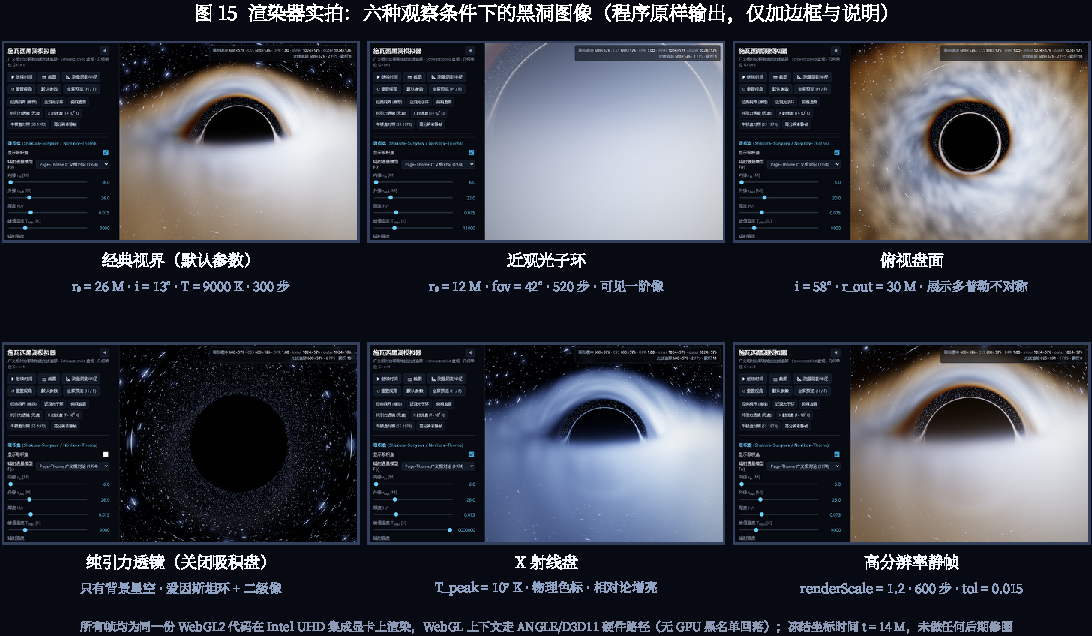
\includegraphics[width=0.99\linewidth]{figures/f19_app_gallery.pdf}
\caption{渲染器实拍：六种观察条件下的黑洞图像（程序原样输出，
仅加边框与说明）。所有帧均为同一份 WebGL2 着色器在
Intel 集成显卡 + 软件光栅化环境下渲染，冻结在 $t=14\M$，
未做任何后期修图。}
\label{fig:19}
\end{figure}

\FloatBarrier

% --------------------------------------------------------------------------- %
\subsection{参数扫描：视线仰角与峰值温度}\label{sec:sweep}

图~\ref{fig:20} 把两个对画面影响最大的参数做成交叉扫描：
视线仰角 $i\in\{6^\circ,22^\circ,50^\circ\}$、
盘峰值温度 $T\in\{3500,9000,30000\}$\,K，
其余参数固定在 $r_0=24\M$、$400$ 步、$tol=0.025$，
并为每个温度单独标定曝光（$1.25/1.00/0.70$）以免色标饱和
掩盖结构。三行之间的差异由几何主导：$i\to0$ 时盘的前后像
在视线上逐渐重合，远侧盘的「上弧」被压缩；
$i\to58^\circ$ 时多普勒不对称把盘分成明显的一明一暗两半。
三列之间的差异由辐射转移主导：峰值温度改变 Planck 谱
与可见光通道的重叠程度，从而改变整体色相与对比度，
但\emph{不}改变增亮图案的几何。

\begin{figure}[t]
\centering
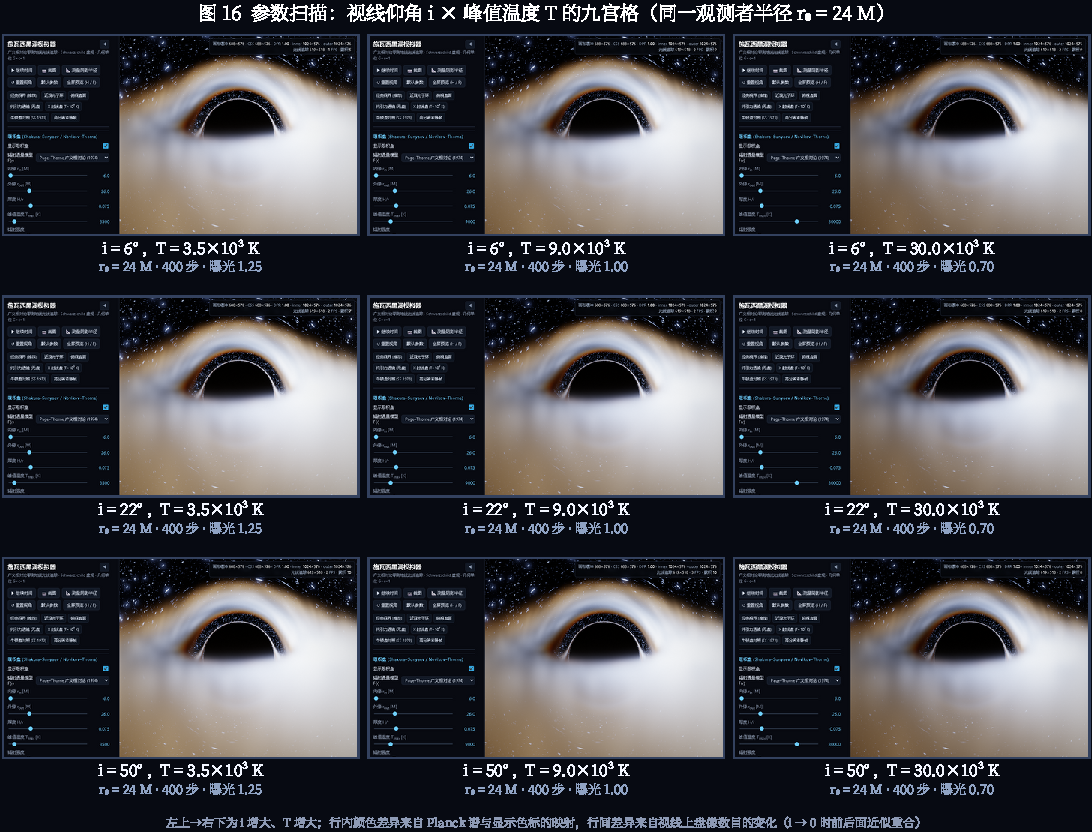
\includegraphics[width=0.99\linewidth]{figures/f20_param_sweep.pdf}
\caption{参数扫描：视线仰角 $i$ 与盘峰值温度 $T$ 的九宫格。
行内（固定 $i$）的颜色差异来自 Planck 谱与显示色标的映射，
行间（固定 $T$）的差异来自视线上盘像的数目与投影形状变化。}
\label{fig:20}
\end{figure}

\FloatBarrier

% --------------------------------------------------------------------------- %
\subsection{视口自适应：侧栏开合与全屏预览下的中心不变量}\label{sec:viewport}

第~\ref{sec:ui} 节说明了实现的处理方式（画布尺寸与面板可见性
彻底解耦），图~\ref{fig:23} 给出了三种状态下的实拍与阴影圆心轨迹。
此处把它作为一项\emph{结果}再点明一次，因为它是一个
「本应平凡、实际却极易出错」的量：
侧栏展开时画布为 $1024\times640$、侧栏收起（\texttt{H} 键全屏预览）
时画布扩展到全部视口、窄窗口下画布为 $900\times560$，
三种状态下由 \texttt{measureShadow()} 回读的阴影圆心
相对画布几何中心的偏差都是 $0$\,px。
由于相机 \texttt{target} 恒为原点、\texttt{enablePan} 为
\texttt{false}，全屏切换前后相机的轨道半径与方位角也逐位相同，
即用户不会在按 \texttt{H} 的一瞬间感到「视角跳了一下」。

% --------------------------------------------------------------------------- %
\subsection{小结}\label{sec:resultssum}

表~\ref{tab:v6summary}（第~\ref{sec:vsum} 节）汇总了六项验证实验的
对照量与判据；本节在其之上补上了三件它在形式上无法覆盖的东西：
一个把帧时间钉在闭式上的\emph{代价模型}
（式~\eqref{eq:costpix}--\eqref{eq:costtol}），
一组对「像阶次」的\emph{完备计数}（图~\ref{fig:16}），
以及把线性响应与对数发散两种渐近分开的\emph{定量标度检验}
（式~\eqref{eq:slopekappa}--\eqref{eq:expx}，图~\ref{fig:25}）。
三者的共同点是：它们都是可以被证伪的陈述，且都给出了残差。
下一节讨论这些残差、这些模型的适用边界，以及本项目
在物理与数值上仍然欠缺的部分。

\FloatBarrier
